\documentclass[ 12pt ]{article}
\usepackage{amsmath, amsthm, amssymb, csquotes, enumitem, graphicx, listings, mathrsfs, xcolor}
\usepackage[margin=0.5in]{geometry}
\graphicspath{ ./ }

\begin{document}

\noindent Landon Fox \\
\noindent CS 487 \\
\noindent April 11, 2021

\begin{center}
	\Large Homework 3: VGG-Lite
\end{center}

\subsection*{Introduction}

We are provided the task of classifying a set of data consisting of pictures of dogs and cats. Some images include the following.
\begin{center}
	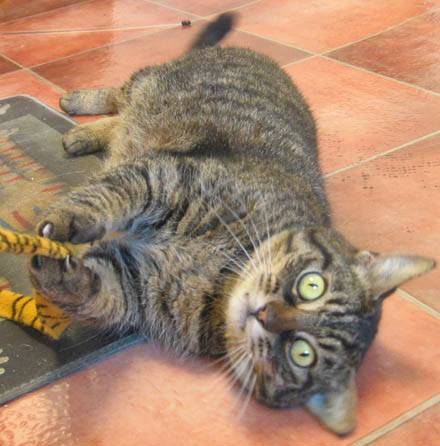
\includegraphics[scale=0.35]{cat.836}
	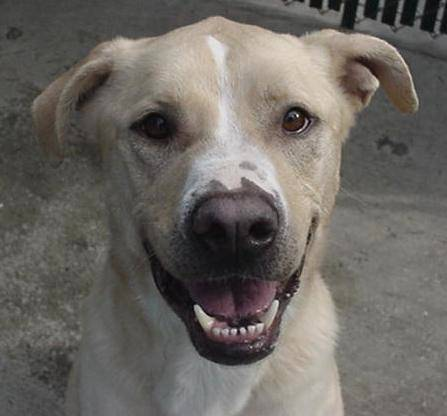
\includegraphics[scale=0.35]{dog.722}
\end{center}
To address this problem we will utilize convolutional neural networks. More specifically, our approach consists of the implementation of a convolutional neural network based on VGGNet
[Simonyan \& Zimmerman].

\subsection*{Network}

The following diagram illustrates the designed and implemented network.
\begin{center}
	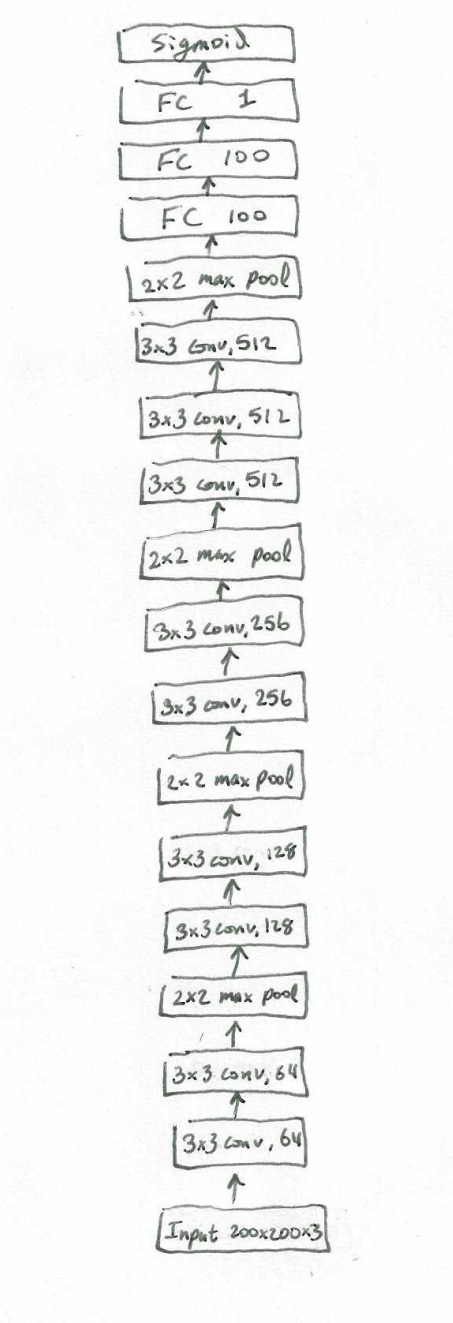
\includegraphics{Capture}
\end{center}
The network is extremely similar to the VGGNet. One slight difference is the use of a sigmoid activation and the difference in the number of layers.

\subsection*{Results}

The accuracy of this model is, in fact, quite poor. Moreover, as illustrated in the accuracy during training,
\begin{lstlisting}[basicstyle=\ttfamily\footnotesize, numbers=left, tabsize=4, frame=single, breaklines=true, postbreak=\mbox{\textcolor{red}{$\hookrightarrow$}\space}]
Epoch 1/5
200/200 [==============================] - 2062s 10s/step - loss: 147.0502 - accuracy: 0.5136 - val_loss: 0.7071 - val_accuracy: 0.5067
Epoch 2/5
200/200 [==============================] - 1824s 9s/step - loss: 0.6825 - accuracy: 0.5661
Epoch 3/5
200/200 [==============================] - 1818s 9s/step - loss: 0.6846 - accuracy: 0.5614
Epoch 4/5
200/200 [==============================] - 1830s 9s/step - loss: 0.6756 - accuracy: 0.5874
Epoch 5/5
200/200 [==============================] - 1839s 9s/step - loss: 0.6652 - accuracy: 0.5982
\end{lstlisting}
we can see it averages around 55\%. I am not aware of the cause of this issue. Due to the strong similarities to the VGGNet architecture, it leads me to believe that there is a mistake
in this implementation. The implementation makes use of the \verb|adam| optimizer and \verb|binary cross entropy| loss. Additionally, here we can see our network summary.
\begin{lstlisting}[basicstyle=\ttfamily\footnotesize, numbers=left, tabsize=4, frame=single, breaklines=true, postbreak=\mbox{\textcolor{red}{$\hookrightarrow$}\space}]
Model: "sequential"
_________________________________________________________________
Layer (type)                 Output Shape              Param #   
=================================================================
conv2d_162 (Conv2D)          (None, None, None, 64)    1792      
_________________________________________________________________
conv2d_163 (Conv2D)          (None, None, None, 64)    36928     
_________________________________________________________________
max_pooling2d_68 (MaxPooling (None, None, None, 64)    0         
_________________________________________________________________
conv2d_164 (Conv2D)          (None, None, None, 128)   73856     
_________________________________________________________________
conv2d_165 (Conv2D)          (None, None, None, 128)   147584    
_________________________________________________________________
max_pooling2d_69 (MaxPooling (None, None, None, 128)   0         
_________________________________________________________________
conv2d_166 (Conv2D)          (None, None, None, 256)   295168    
_________________________________________________________________
conv2d_167 (Conv2D)          (None, None, None, 256)   590080    
_________________________________________________________________
max_pooling2d_70 (MaxPooling (None, None, None, 256)   0         
_________________________________________________________________
conv2d_168 (Conv2D)          (None, None, None, 512)   1180160   
_________________________________________________________________
conv2d_169 (Conv2D)          (None, None, None, 512)   2359808   
_________________________________________________________________
conv2d_170 (Conv2D)          (None, None, None, 512)   2359808   
_________________________________________________________________
max_pooling2d_71 (MaxPooling (None, None, None, 512)   0         
_________________________________________________________________
flatten_14 (Flatten)         (None, None)              0         
_________________________________________________________________
dense_42 (Dense)             (None, 100)               7372900   
_________________________________________________________________
dense_43 (Dense)             (None, 100)               10100     
_________________________________________________________________
dense_44 (Dense)             (None, 1)                 101       
_________________________________________________________________
activation_14 (Activation)   (None, 1)                 0         
=================================================================
Total params: 14,428,285
Trainable params: 14,428,285
Non-trainable params: 0
\end{lstlisting}

\end{document}
